\documentclass[xcolor=svgnames]{beamer}
\usepackage[utf8]{inputenc}
\usepackage[english]{babel}

\newcommand{\semitransp}[2][35]{\color{fg!#1}#2}
\usepackage{wrapfig}
\usepackage{graphicx, booktabs}
\usepackage[autolanguage]{numprint}

\usetheme{Proso}

\title[Adaptivní výukové systémy]{Adaptivní výukové systémy}
\author{Vít Stanislav, Jan Papoušek, Jiří Řihák}
\institute{Fakulta informatiky Masarykovy univerzity}      % Enter your institute name between curly braces
\date{10. 2. 2016}

\begin{document}
% --------------------------- SLIDE --------------------------------------------
\frame[plain]{\titlepage}
% ------------------------------------------------------------------------------
% --------------------------- SLIDE --------------------------------------------
\begin{frame}
  \huge{Co jsou adaptivní výukové systémy?}
\end{frame}
% ------------------------------------------------------------------------------
% --------------------------- SLIDE --------------------------------------------
\begin{frame}
	\frametitle{Příklad}
   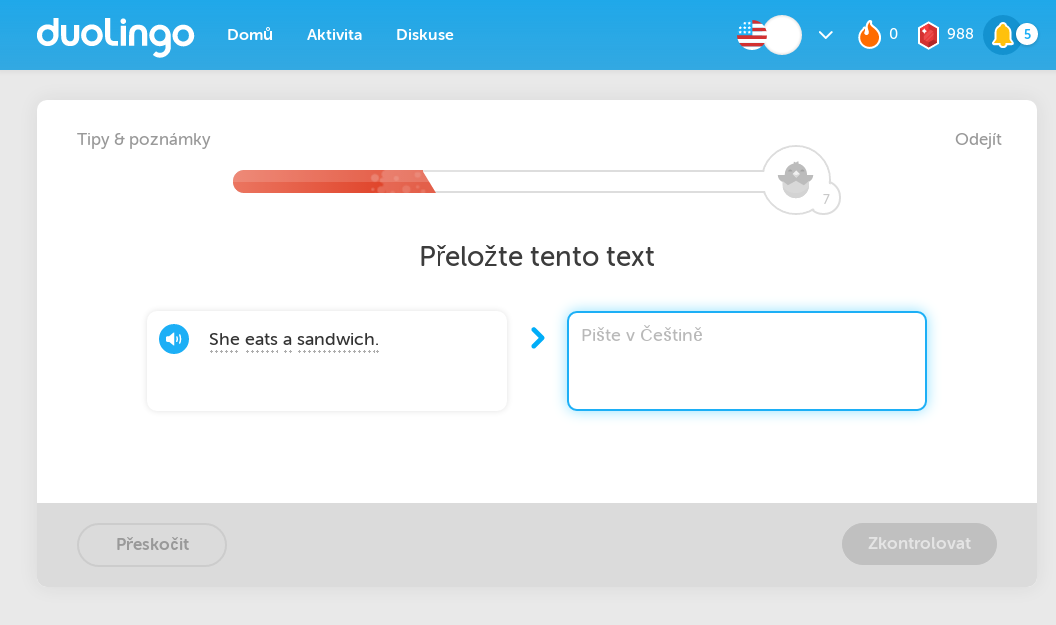
\includegraphics[width=\textwidth]{img/duolingo-practice}
\end{frame}
% ------------------------------------------------------------------------------
% --------------------------- SLIDE --------------------------------------------
\begin{frame}
	\frametitle{Příklad}
   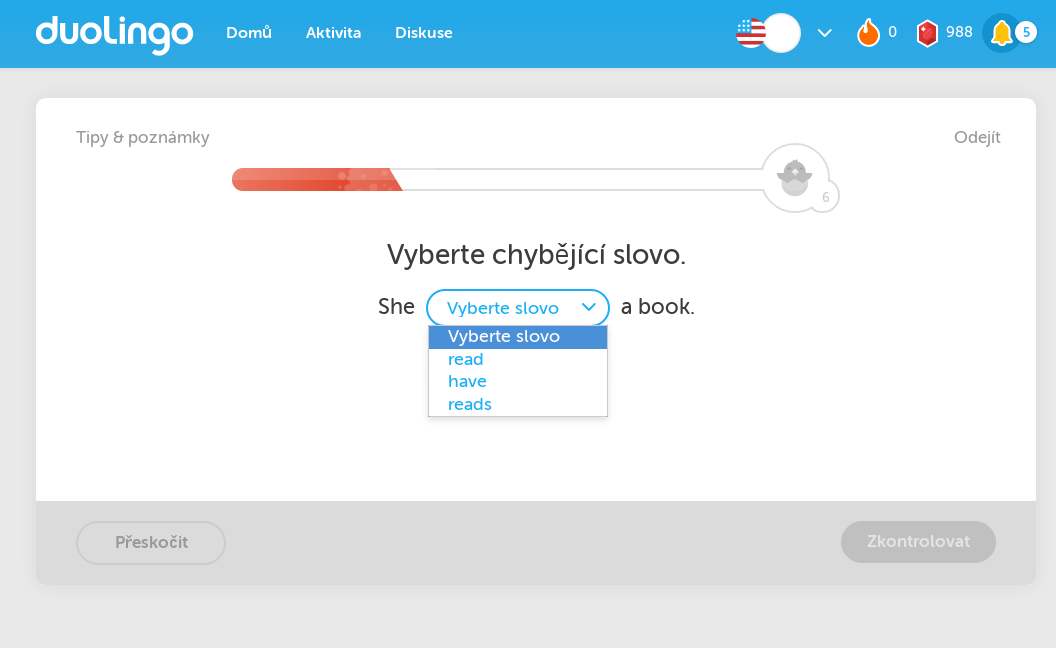
\includegraphics[width=\textwidth]{img/duolingo-practice-2}
\end{frame}
% ------------------------------------------------------------------------------
% --------------------------- SLIDE --------------------------------------------
\begin{frame}
	\frametitle{Příklad: Duolingo}
	\hspace{0.1\textwidth}
   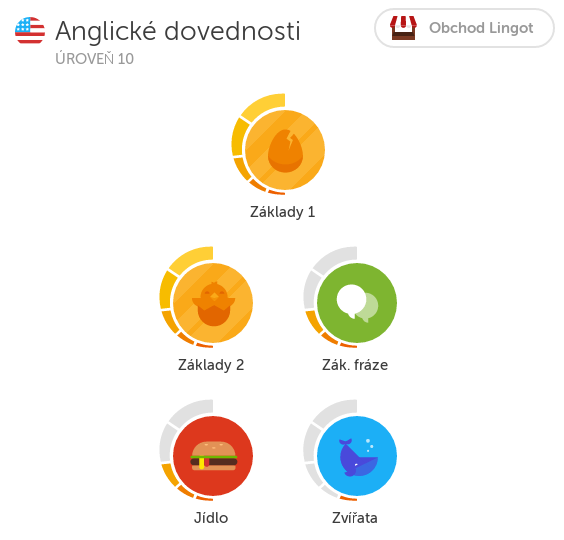
\includegraphics[width=0.8\textwidth]{img/duolingo-skills}
\end{frame}
% ------------------------------------------------------------------------------
% --------------------------- SLIDE --------------------------------------------
\begin{frame}
	\frametitle{Naše systémy}
   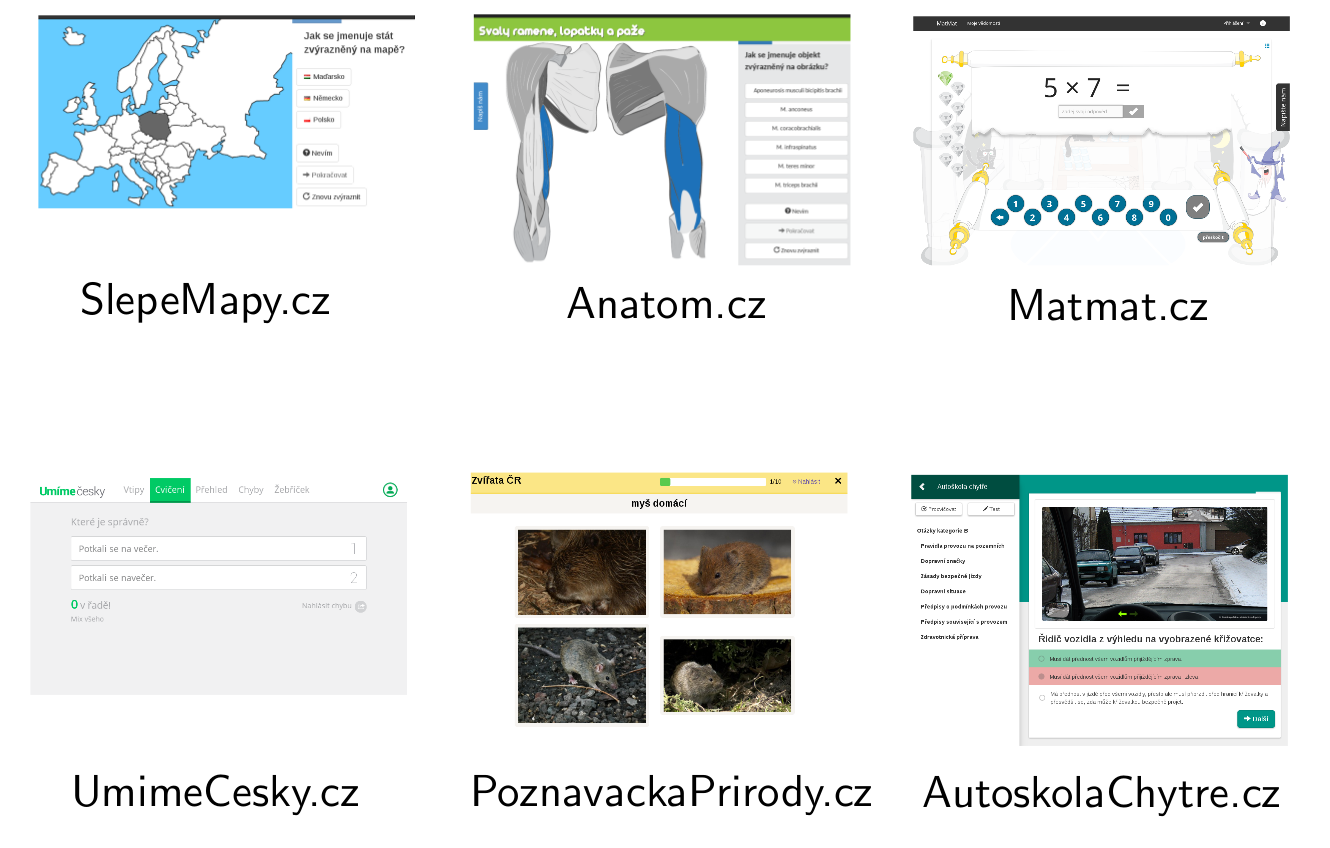
\includegraphics[width=\textwidth]{img/system-grid}
\end{frame}
% ------------------------------------------------------------------------------
% --------------------------- SLIDE --------------------------------------------
\begin{frame}
	\frametitle{SlepeMapy.cz}
   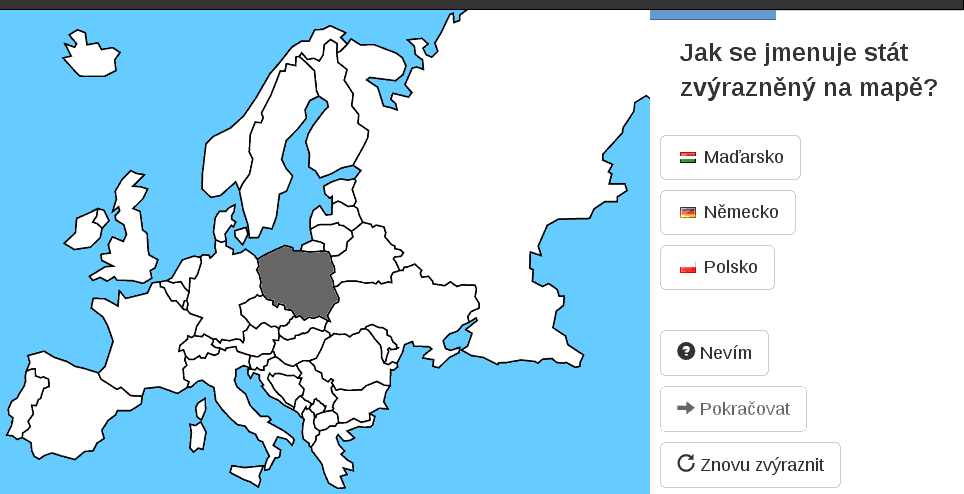
\includegraphics[width=\textwidth]{img/practice-example-cs}
\end{frame}
% ------------------------------------------------------------------------------
% --------------------------- SLIDE --------------------------------------------
\begin{frame}
	\frametitle{SlepeMapy.cz}
   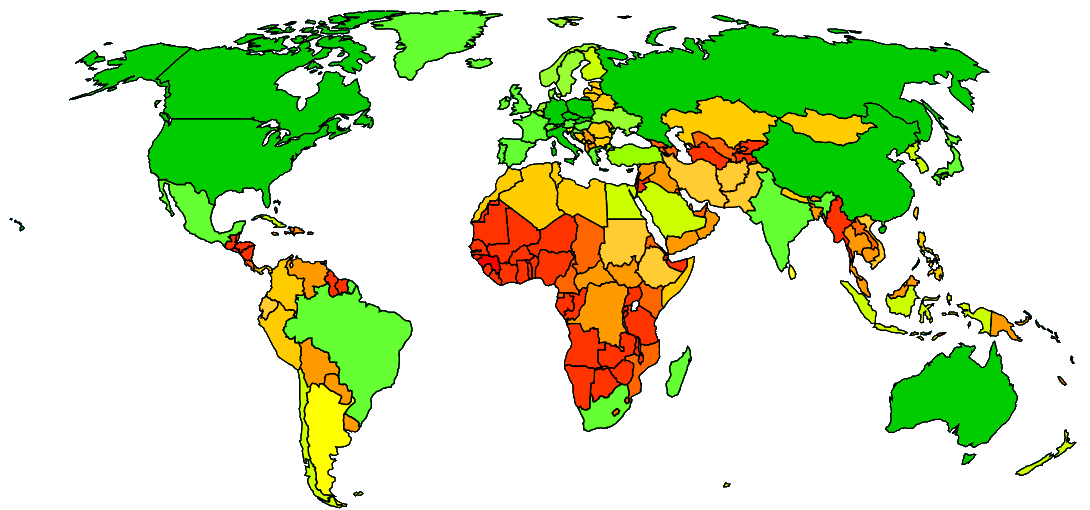
\includegraphics[width=\textwidth]{img/knowledge-map}
\end{frame}
% ------------------------------------------------------------------------------
% --------------------------- SLIDE --------------------------------------------
\begin{frame}
	\frametitle{Anatom.cz}
   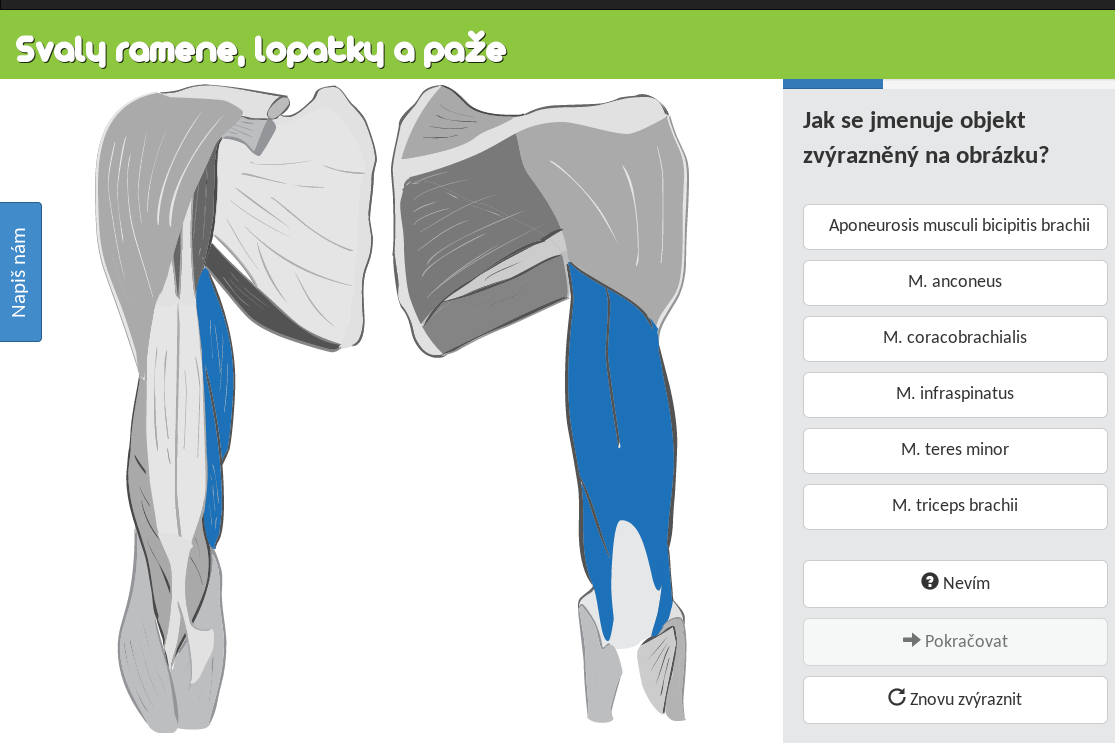
\includegraphics[width=\textwidth]{img/anatom-practice-cs}
\end{frame}
% ------------------------------------------------------------------------------
% --------------------------- SLIDE --------------------------------------------
\begin{frame}
	\frametitle{Matmat.cz}
   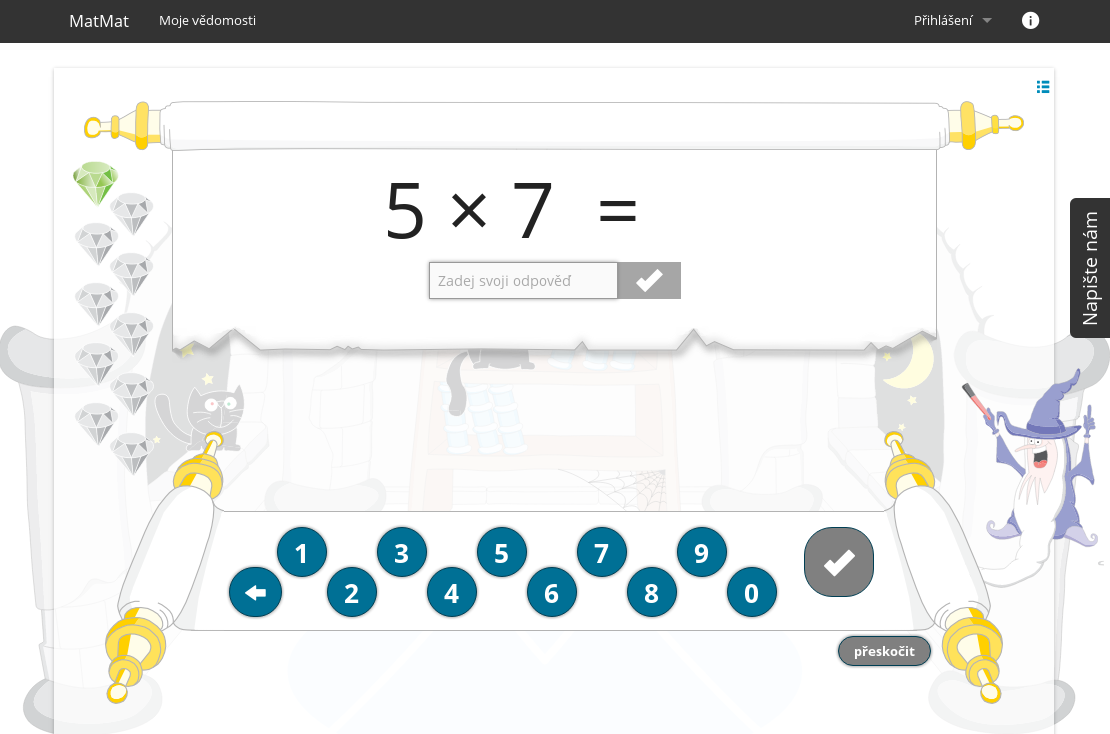
\includegraphics[width=\textwidth]{img/matmat}
\end{frame}
% ------------------------------------------------------------------------------
% --------------------------- SLIDE --------------------------------------------
\begin{frame}
	\frametitle{UmimeCesky.cz}
   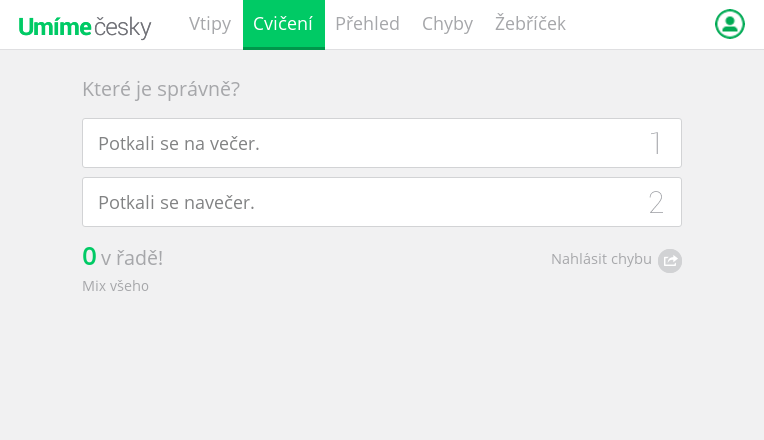
\includegraphics[width=\textwidth]{img/umimecesky}
\end{frame}
% ------------------------------------------------------------------------------
% --------------------------- SLIDE --------------------------------------------
\begin{frame}
	\frametitle{PoznavackaPrirody.cz}
   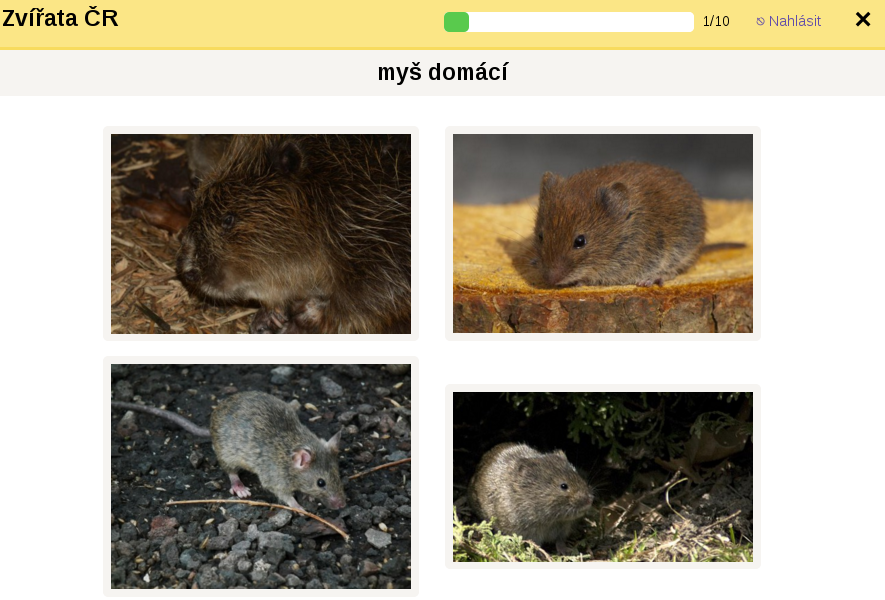
\includegraphics[width=\textwidth]{img/poznavackaprirody}
\end{frame}
% ------------------------------------------------------------------------------
% --------------------------- SLIDE --------------------------------------------
\begin{frame}
	\frametitle{AutoskolaChytre.cz}
   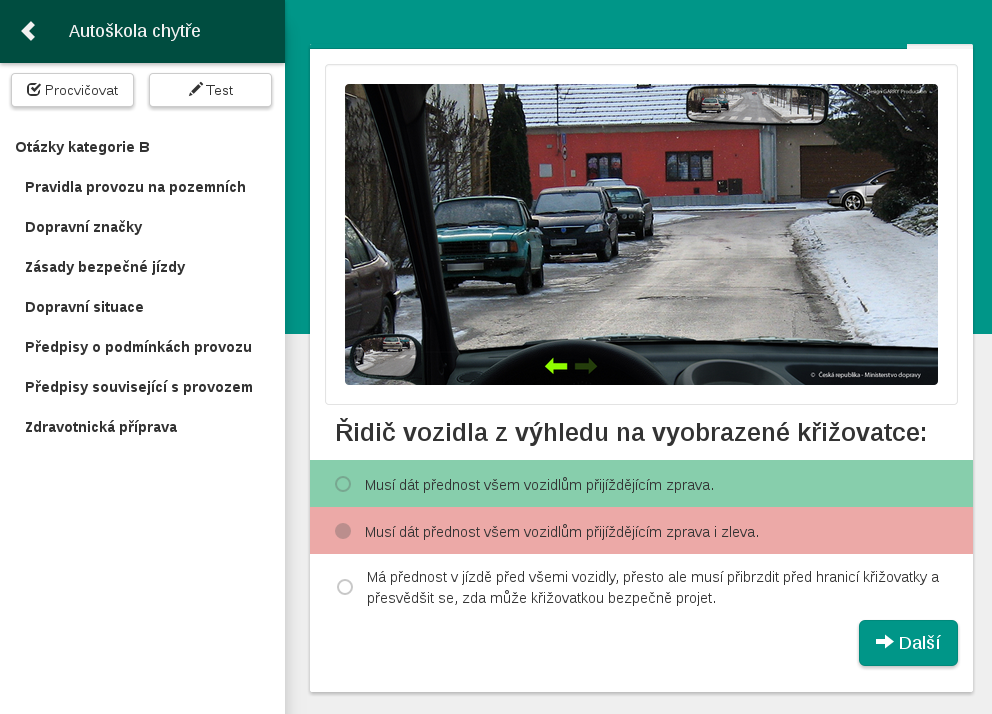
\includegraphics[width=\textwidth]{img/autoskola}
\end{frame}
% ------------------------------------------------------------------------------
% --------------------------- SLIDE --------------------------------------------
\begin{frame}
	\frametitle{Naše systémy}
   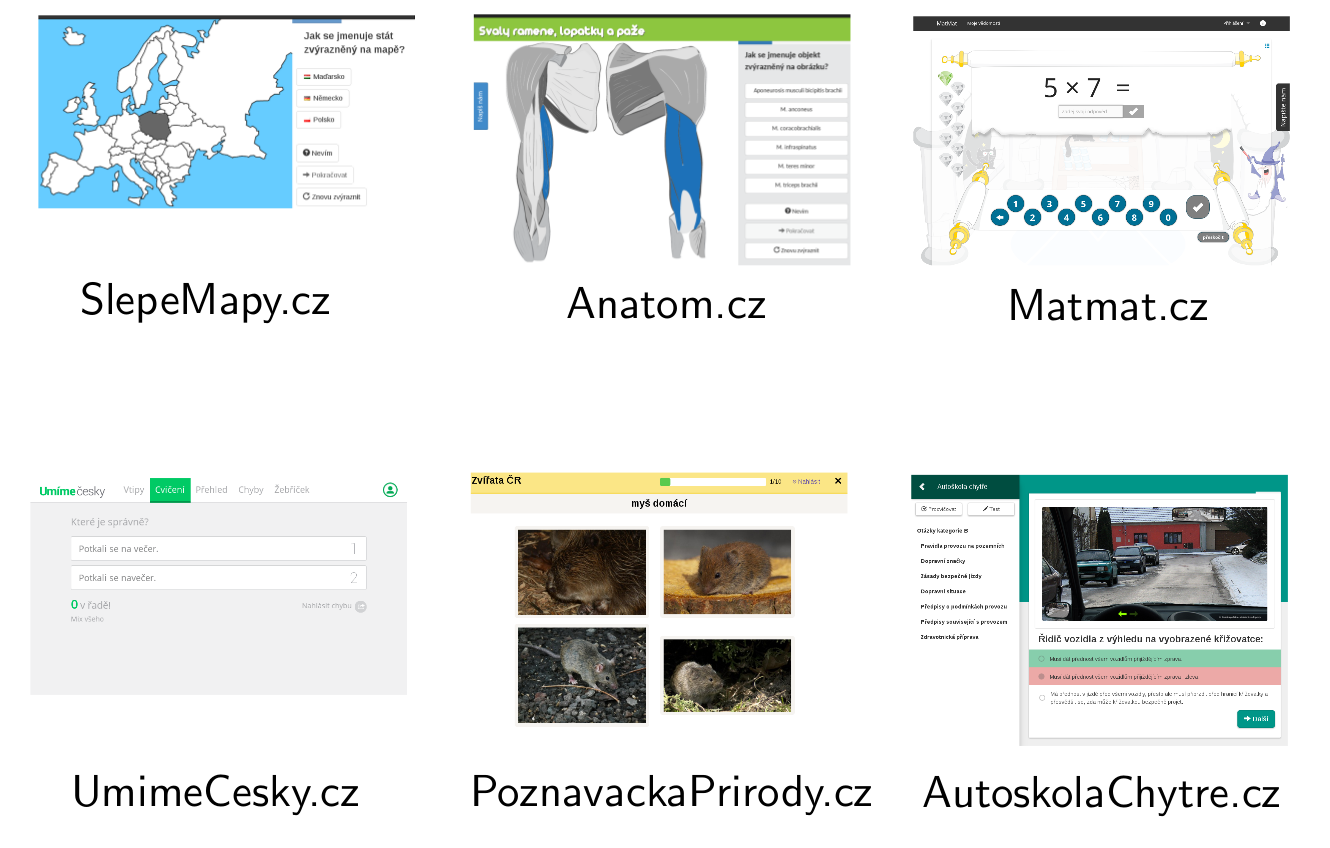
\includegraphics[width=\textwidth]{img/system-grid}
\end{frame}
% ------------------------------------------------------------------------------
% --------------------------- SLIDE --------------------------------------------
\begin{frame}
	\begin{center}
		\Huge{Jak se to chová uvnitř?}
	\end{center}
\end{frame}
% ------------------------------------------------------------------------------
% --------------------------- SLIDE --------------------------------------------
\begin{frame}
	\frametitle{Co vlastně víme o uživatelích?}
	
\includegraphics[width=\textwidth]{img/data_collection}

	\pause
	\begin{columns}
		\begin{column}{.5\textwidth}
			Slepé mapy
			\begin{itemize}
				\item 19 000 000 odpovědí
			\end{itemize}
			Anatom
			\begin{itemize}
				\item 400 000 odpovědí
			\end{itemize}
		\end{column}
		\begin{column}{.5\textwidth}
			Umíme česky
			\begin{itemize}
				\item 400 000 odpovědí
			\end{itemize}
			MatMat
			\begin{itemize}
				\item 200 000 odpovědí
			\end{itemize}
		\end{column}
	\end{columns}
\end{frame}
% ------------------------------------------------------------------------------
% --------------------------- SLIDE --------------------------------------------
\begin{frame}
	\frametitle{Čeho se snažíme dosáhnout?}
	\begin{columns}
		\begin{column}{.4\textwidth}
			\begin{center}
				
\includegraphics[width=\textwidth]{img/balance}
			\end{center}
		\end{column}
		\begin{column}{.6\textwidth}
			\pause
			vhodná obtížnost
			\begin{itemize}
				\item Jaká přesně?
				\item u šachistů optimální cca 20\% pravděpodobnost výhry
			\end{itemize}
			různé reprezentace, počet možností, \ldots
		\end{column}
	\end{columns}
\end{frame}
% ------------------------------------------------------------------------------
% --------------------------- SLIDE --------------------------------------------
\begin{frame}
	\frametitle{Anatom: nasbíraná data}
	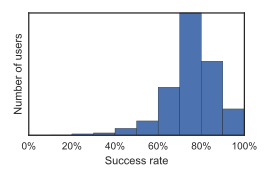
\includegraphics[width=\textwidth]{img/user_success_hist}
\end{frame}
% ------------------------------------------------------------------------------
% --------------------------- SLIDE --------------------------------------------
\begin{frame}
	\frametitle{Model znalosti uživatele}
	\textbf{obtížnost položky v systému}
	\begin{itemize}
		\item Ghana je těžší než Egypt
	\end{itemize}
	\textbf{vstupní znalosti uživatele}
	\begin{itemize}
		\item prokrastinující dospělý vs. dítě ze základní školy
	\end{itemize}
	\textbf{aktuální znalost uživatele pro danou položku}
	\begin{itemize}
		\item učení, zapomínání, \ldots
	\end{itemize}

	\pause
	\bigskip
	\hrule

	\medskip
	existuje mnoho různých přístupů:
	\begin{itemize}
		\item Item Response Theory
		\item Bayesian Knowledge Tracing
		\item Performance Factor Analysis
		\item \ldots
	\end{itemize}
\end{frame}
% ------------------------------------------------------------------------------
% --------------------------- SLIDE --------------------------------------------
\begin{frame}
	\frametitle{Model znalosti uživatele}
	\begin{center}
	{\Huge $P(correct|u, i) = ?$}
	\end{center}
\end{frame}
% ------------------------------------------------------------------------------
% --------------------------- SLIDE --------------------------------------------
\begin{frame}
	\frametitle{Na co se ptát?}
	\begin{columns}
		\begin{column}{.5\textwidth}
			\begin{center}
				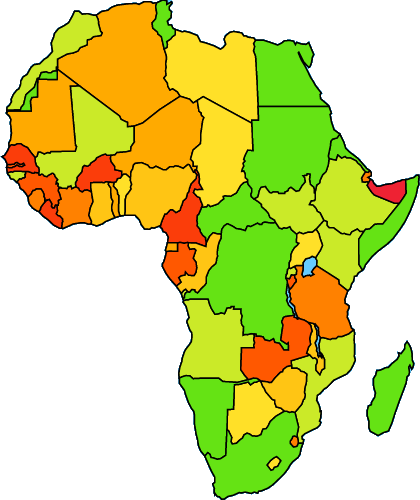
\includegraphics[width=\textwidth]{img/africa_me}
			\end{center}
		\end{column}
		\begin{column}{.5\textwidth}
		pro uživatele a položku známe:
			\begin{itemize}
				\item \textbf{obtížnost}
				\item počet odpovědí
				\item čas od poslední odpovědi
				\item \ldots
			\end{itemize}
		vybereme nejlepšího kandidáta
		\end{column}
	\end{columns}
\end{frame}
% ------------------------------------------------------------------------------
% --------------------------- SLIDE --------------------------------------------
\begin{frame}
	\frametitle{Jak se ptát?}
	\begin{columns}
		\begin{column}{.5\textwidth}
			\begin{center}
				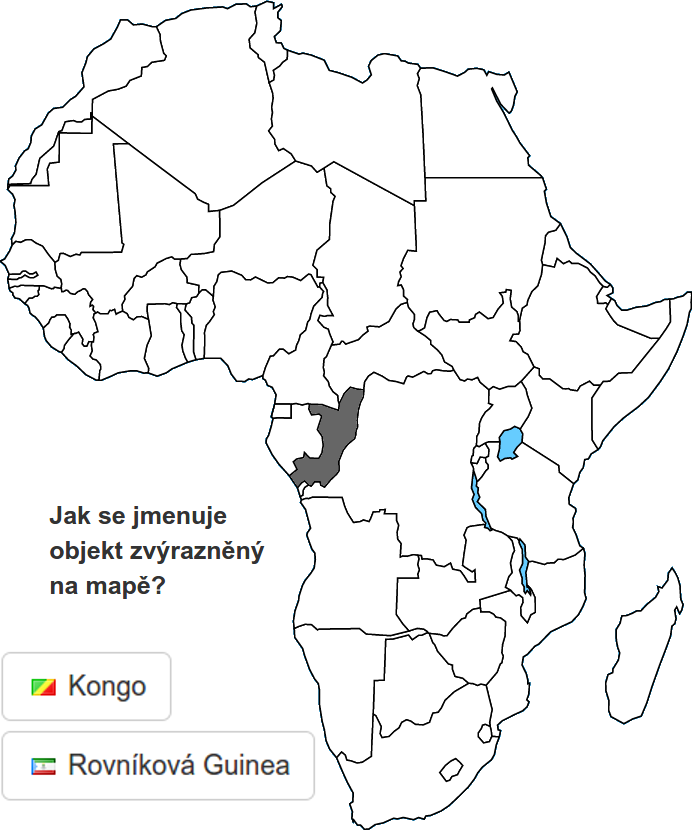
\includegraphics[width=\textwidth]{img/slepemapy_mcq}
			\end{center}
		\end{column}
		\begin{column}{.5\textwidth}
			\begin{center}
				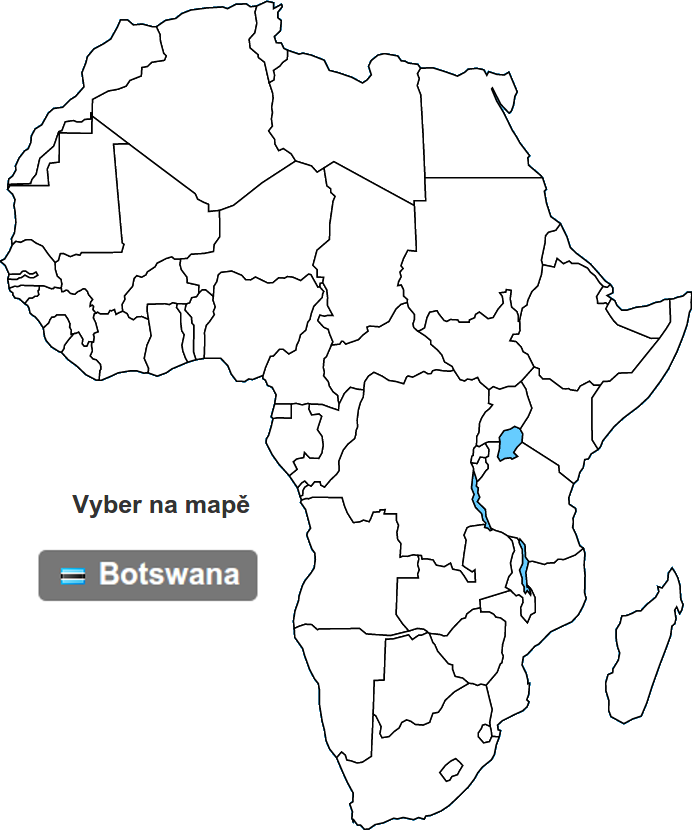
\includegraphics[width=\textwidth]{img/slepemapy_open}
			\end{center}
		\end{column}
	\end{columns}
\end{frame}
% ------------------------------------------------------------------------------
% --------------------------- SLIDE --------------------------------------------
\begin{frame}
	\frametitle{Jak se ptát?}
	\begin{center}
		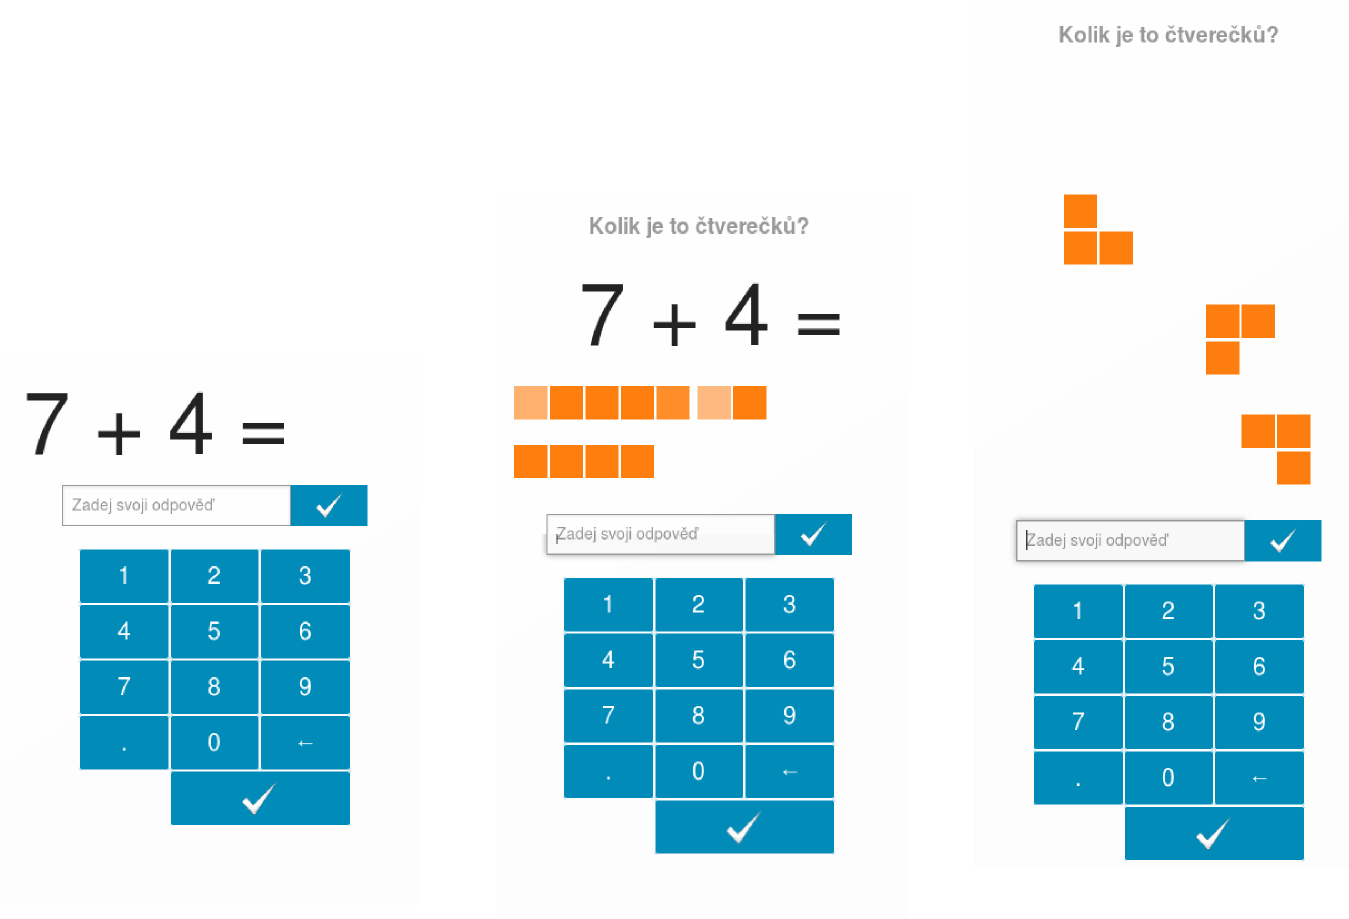
\includegraphics[width=.8\textwidth]{img/matmat_questions}
	\end{center}
\end{frame}
% ------------------------------------------------------------------------------
% --------------------------- SLIDE --------------------------------------------
\begin{frame}
	\frametitle{AB experimenty}
	\begin{itemize}
		\item uživatele rozdělujeme náhodně do skupin
		\item každá skupině poskytujeme jinou verzi systému
	\end{itemize}
	\begin{center}
		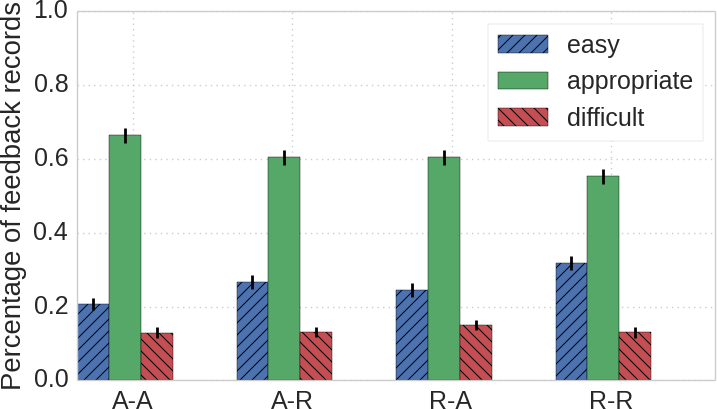
\includegraphics[width=.8\textwidth]{img/feedback}
	\end{center}
\end{frame}
% ------------------------------------------------------------------------------
% --------------------------- SLIDE --------------------------------------------
\begin{frame}
	\frametitle{Zpětná vazba}
	\begin{center}
		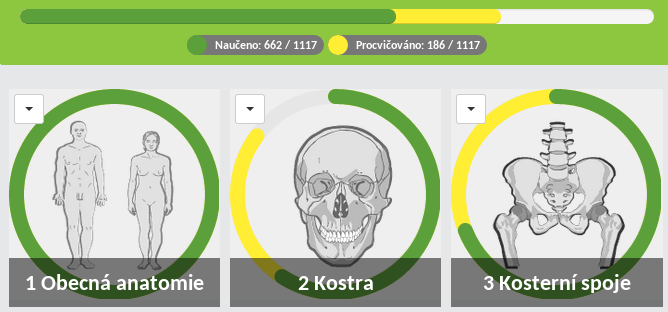
\includegraphics[width=.8\textwidth]{img/knowledge_feedback_overview}
	\end{center}
	\pause
	\begin{itemize}
		\item Některé položky uživatel nikdy neuvidí.
			\begin{itemize}
				\item příliš lehké / příliš těžké
			\end{itemize}
		\item Kdy prohlásit nějakou položku za naučenou?
			\begin{itemize}
				\item model znalosti uživatele
			\end{itemize}
	\end{itemize}
\end{frame}
% ------------------------------------------------------------------------------
% --------------------------- SLIDE --------------------------------------------
\begin{frame}
	\frametitle{Zpětná vazba}
	\begin{center}
		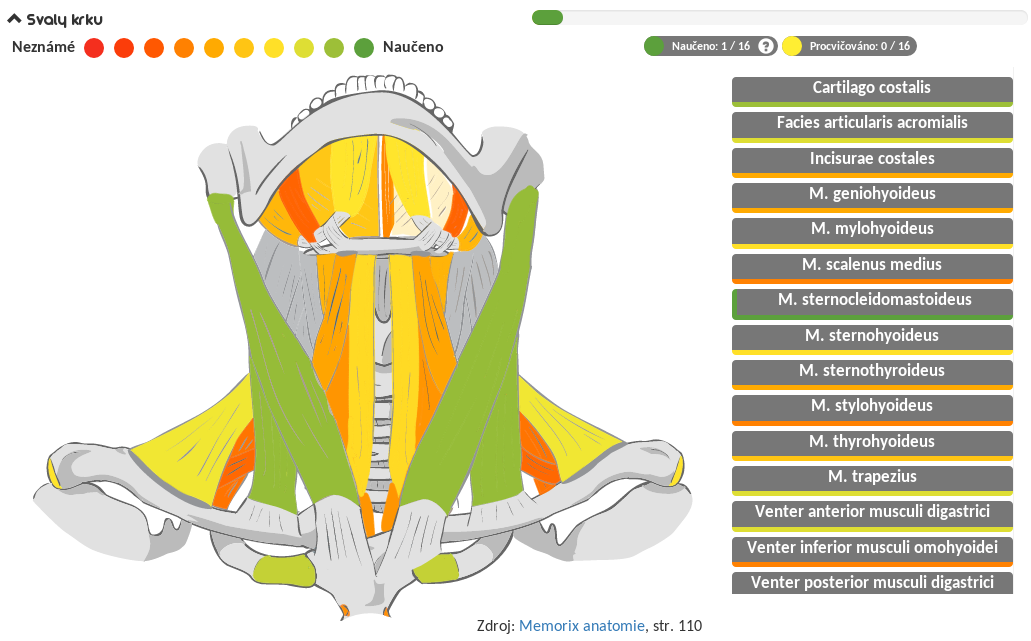
\includegraphics[width=\textwidth]{img/knowledge_feedback_detail}
	\end{center}
\end{frame}
% ------------------------------------------------------------------------------
% --------------------------- SLIDE --------------------------------------------
\begin{frame}
	\begin{center}
		\Huge{Co nám data mohou říci?}
	\end{center}
\end{frame}
% ------------------------------------------------------------------------------
% --------------------------- SLIDE --------------------------------------------
\begin{frame}
	\frametitle{Co nám data mohou říci?}
	
\includegraphics[width=\textwidth]{img/experiments_intro}
\end{frame}
% ------------------------------------------------------------------------------
% --------------------------- SLIDE --------------------------------------------
\begin{frame}
	\frametitle{Obtížnost - malá násobilka}
	\begin{center}
		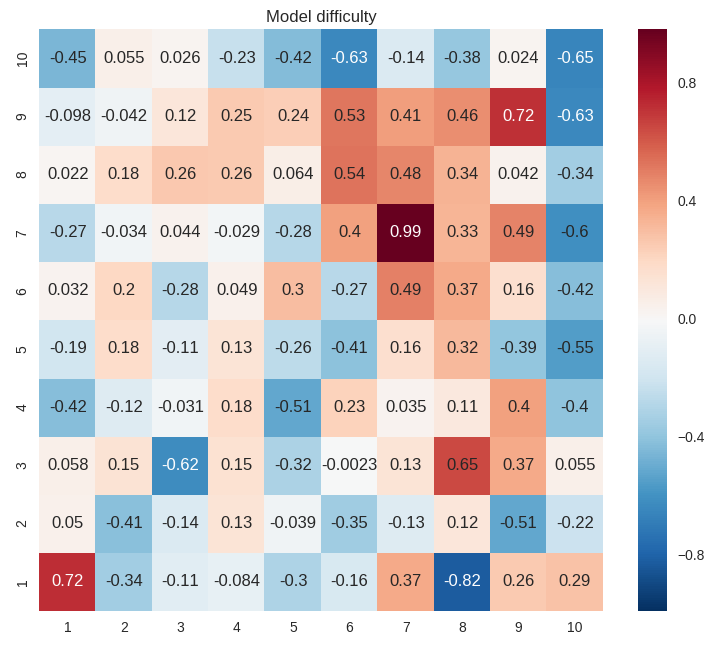
\includegraphics[width=0.8\textwidth]{img/multiplication_difficulty}
	\end{center}
\end{frame}
% ------------------------------------------------------------------------------
% --------------------------- SLIDE --------------------------------------------
\begin{frame}
	\frametitle{Špatné odpovědi - dělení}
	\begin{center}
		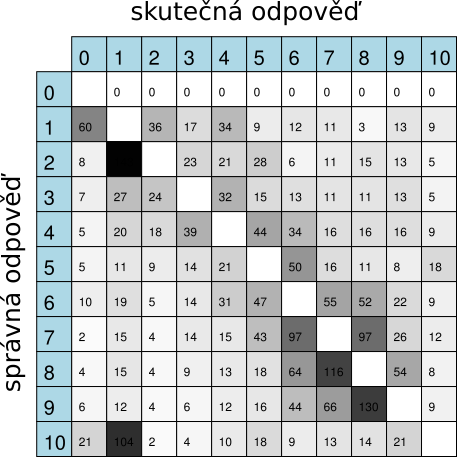
\includegraphics[width=0.7\textwidth]{img/confusion_table_10_div.png}
	\end{center}
\end{frame}
% ------------------------------------------------------------------------------
% --------------------------- SLIDE --------------------------------------------
\begin{frame}
	\frametitle{Co se plete v Evropě?}
	\begin{center}
		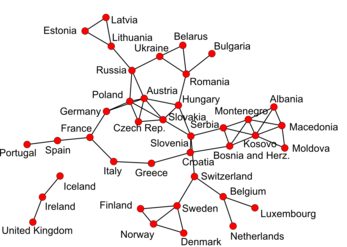
\includegraphics[width=0.7\textwidth]{img/europe-graph-clusters.png}
	\end{center}
\end{frame}
% ------------------------------------------------------------------------------
% --------------------------- SLIDE --------------------------------------------
\begin{frame}
	\frametitle{Co se plete v Evropě?}
	\begin{center}
		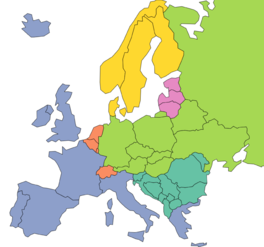
\includegraphics[width=0.5\textwidth]{img/europe-graph-clusters2.png}
	\end{center}
\end{frame}
% ------------------------------------------------------------------------------
% --------------------------- SLIDE --------------------------------------------
\begin{frame}
	\frametitle{Které otázky jsou podobné?}
	\begin{center}
		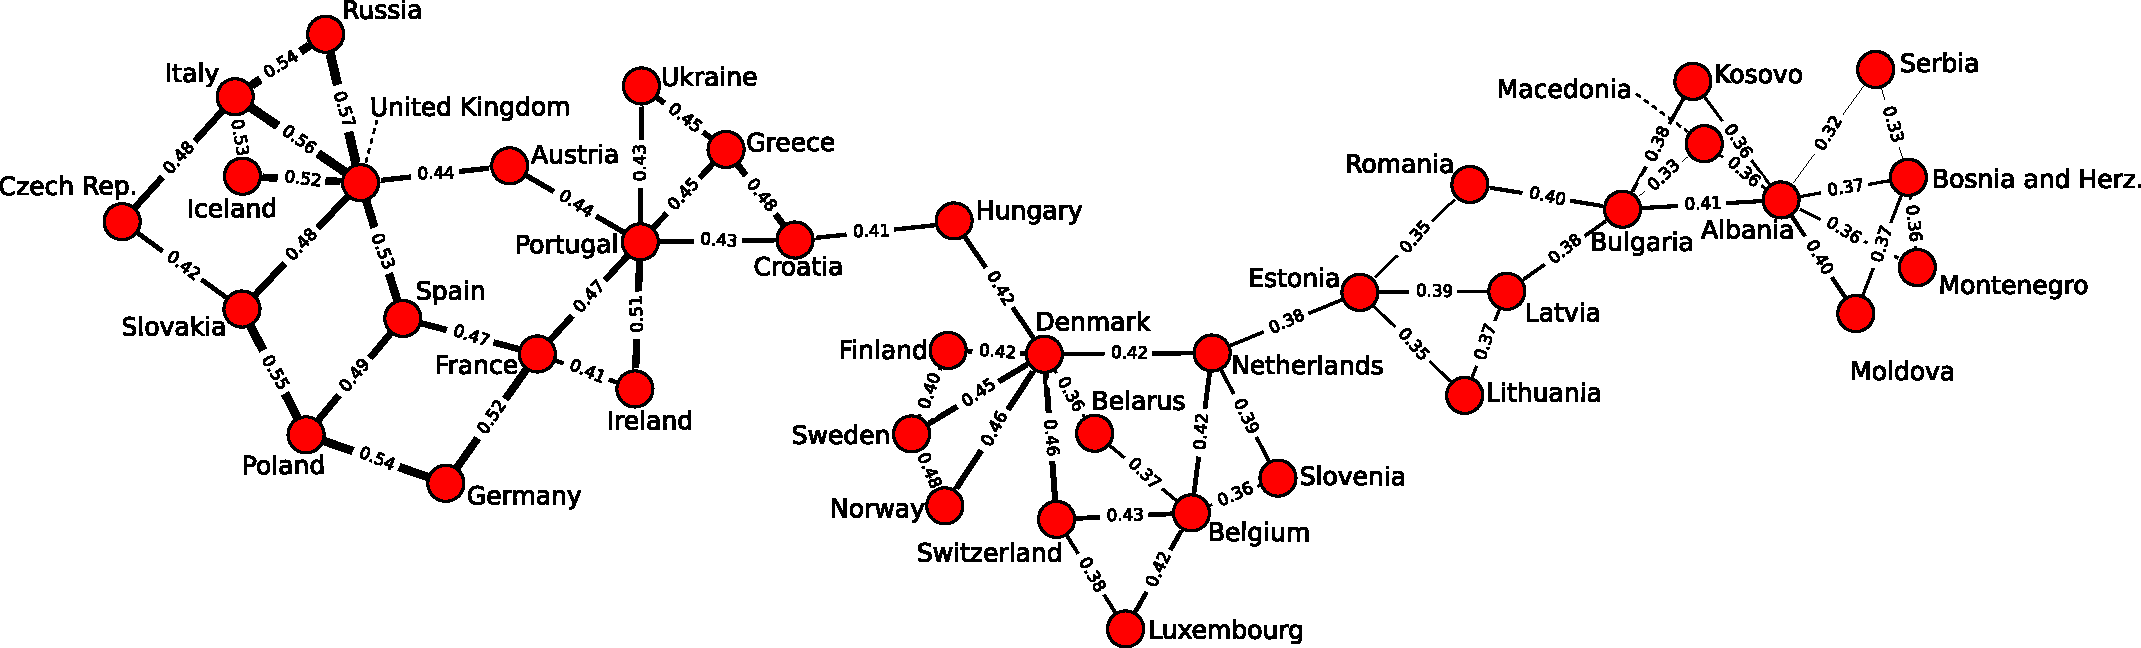
\includegraphics[width=\textwidth]{img/europe-graph}
	\end{center}
\end{frame}
% ------------------------------------------------------------------------------
% --------------------------- SLIDE --------------------------------------------
\begin{frame}
	\frametitle{Co nám podobnosti mohou říci?}
	\begin{center}
		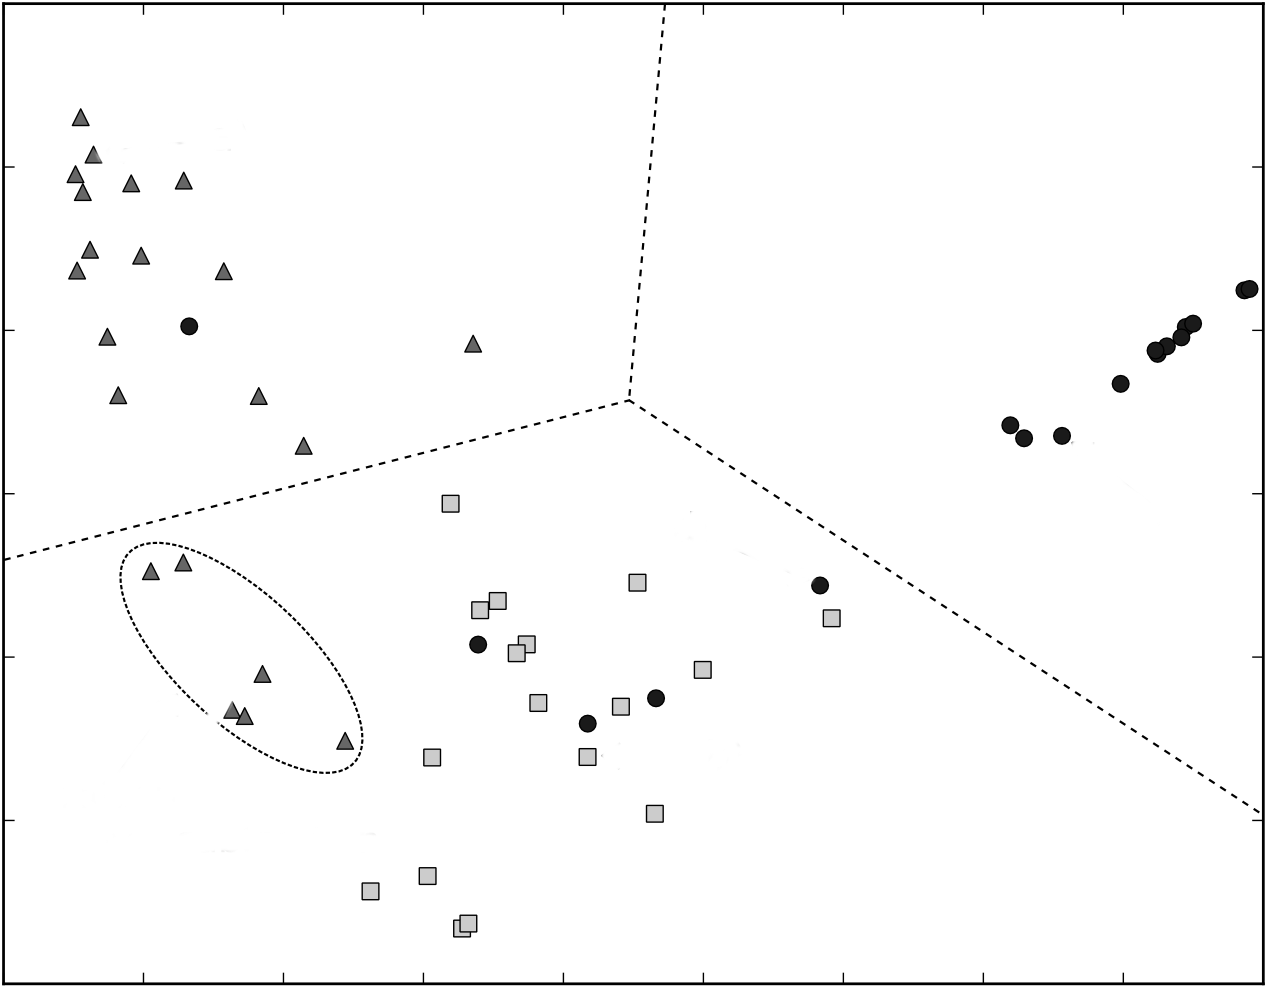
\includegraphics[width=0.8\textwidth]{img/binar2.png}
	\end{center}
\end{frame}
% ------------------------------------------------------------------------------
% --------------------------- SLIDE --------------------------------------------
\begin{frame}
	\frametitle{Jak rychle se uživatelé učí?}
	\begin{center}
		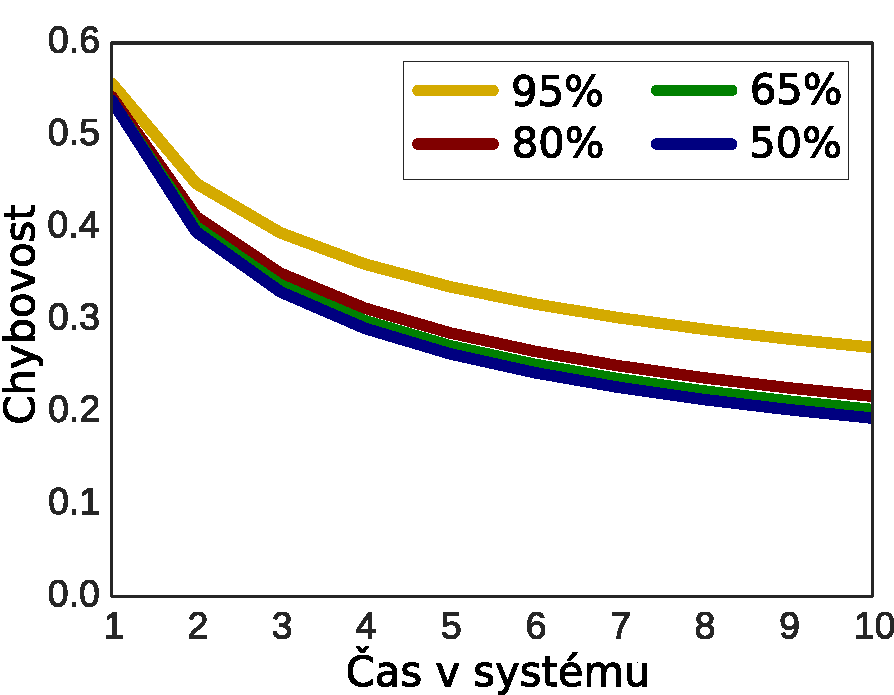
\includegraphics[width=0.8\textwidth]{img/target_difficulty_context_learning_slope}
	\end{center}
\end{frame}
% ------------------------------------------------------------------------------
% --------------------------- SLIDE --------------------------------------------
\begin{frame}
	\frametitle{Jak dlouho uživatelé vydrží v systému?}
	\begin{center}
		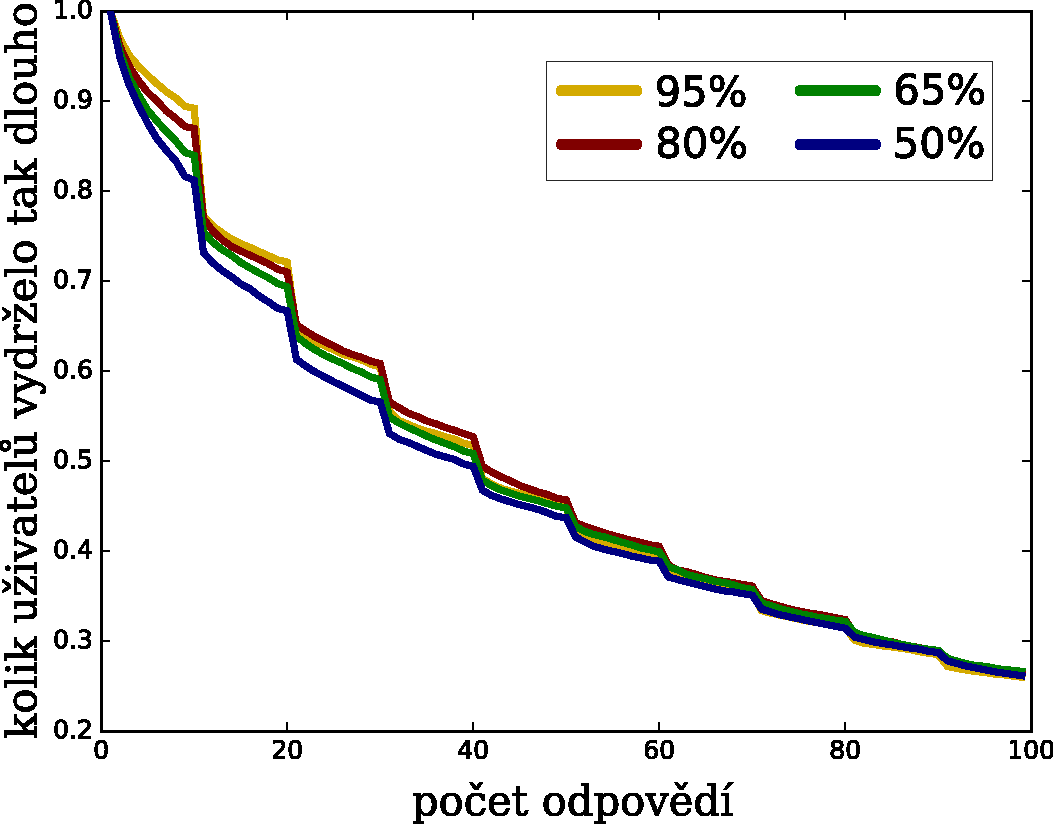
\includegraphics[width=0.8\textwidth]{img/drop-off}
	\end{center}
\end{frame}
% ------------------------------------------------------------------------------
% --------------------------- SLIDE --------------------------------------------
\begin{frame}
	\begin{center}
		\Huge{Kde se bere náš obsah?}
	\end{center}
\end{frame}
% ------------------------------------------------------------------------------
% --------------------------- SLIDE --------------------------------------------
\begin{frame}
	\frametitle{Zdroje obsahu}

	\begin{itemize}
	    \item Otevřené zdroje
	    \item Hlášení chyb uživateli
	    \item Umíme česky -- tvorba obsahu lingvistou
		\item Slepé mapy -- mapy, překlady (němčina, španělština, ruština,~\dots)
		\item Anatom -- obsah kompletně vytvořen experty (Memorix, doktoři, medici)
	\end{itemize}
\end{frame}
% ---------------------------------------------------------------------------
% --------------------------- SLIDE --------------------------------------------
\begin{frame}
    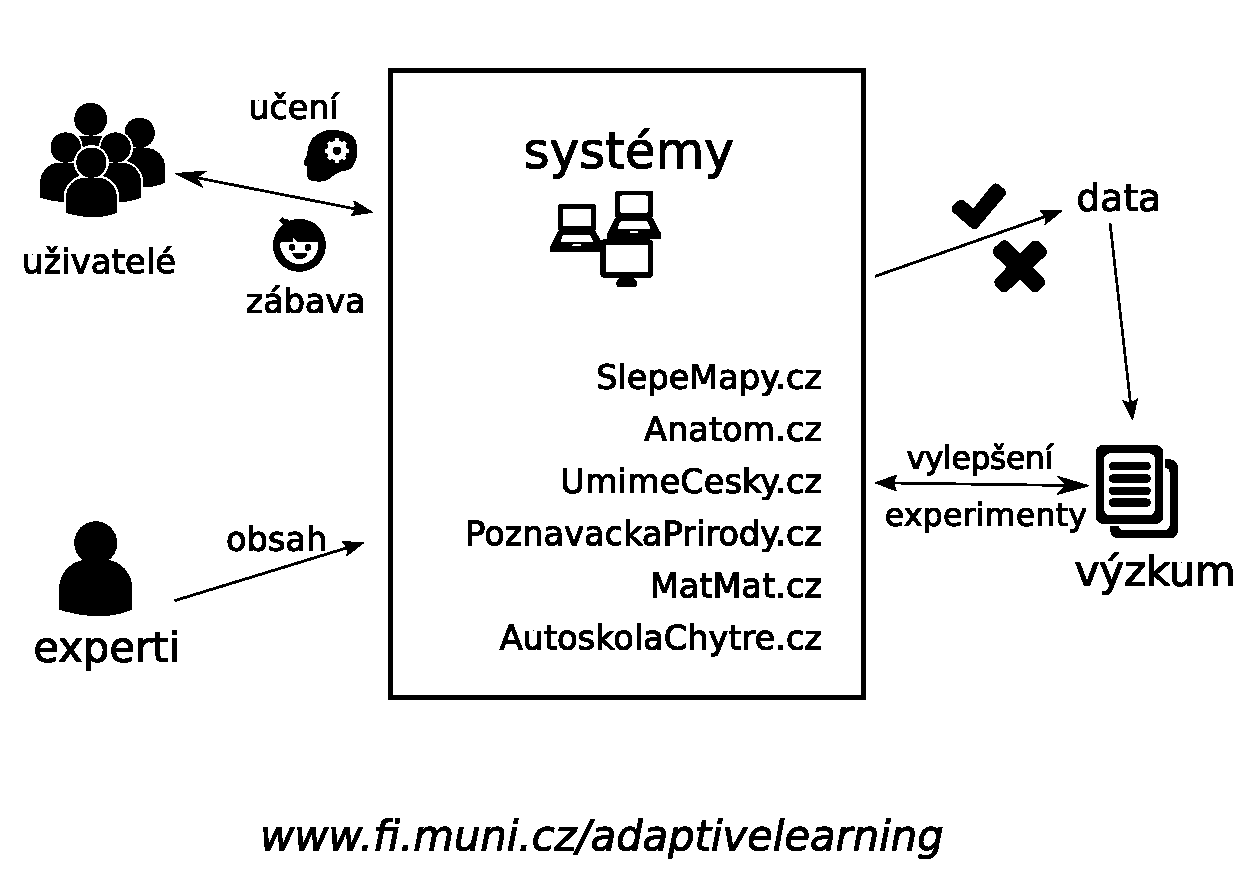
\includegraphics[width=\textwidth]{img/summary}
\end{frame}
% ------------------------------------------------------------------------------
\end{document}
